% Für Bindekorrektur als optionales Argument "BCORfaktormitmaßeinheit", dann
% sieht auch Option "twoside" vernünftig aus
% Näheres zu "scrartcl" bzw. "scrreprt" und "scrbook" siehe KOMA-Skript Doku
\documentclass[12pt,a4paper,titlepage,headinclude,bibtotoc]{scrartcl}


%---- Allgemeine Layout Einstellungen ------------------------------------------

% Für Kopf und Fußzeilen, siehe auch KOMA-Skript Doku
\usepackage[komastyle]{scrpage2}
\pagestyle{scrheadings}
\automark[section]{chapter}
\setheadsepline{0.5pt}[\color{black}]

%keine Einrückung
\parindent0pt

%Einstellungen für Figuren- und Tabellenbeschriftungen
\setkomafont{captionlabel}{\sffamily\bfseries}
\setcapindent{0em}

\usepackage{caption}

%---- Weitere Pakete -----------------------------------------------------------
% Die Pakete sind alle in der TeX Live Distribution enthalten. Wichtige Adressen
% www.ctan.org, www.dante.de

% Sprachunterstützung
\usepackage[ngerman]{babel}

% Benutzung von Umlauten direkt im Text
% entweder "latin1" oder "utf8"
\usepackage[utf8]{inputenc}

% Pakete mit Mathesymbolen und zur Beseitigung von Schwächen der Mathe-Umgebung
\usepackage{latexsym,exscale,amssymb,amsmath}

% Weitere Symbole
\usepackage[nointegrals]{wasysym}
\usepackage{eurosym}

% Anderes Literaturverzeichnisformat
%\usepackage[square,sort&compress]{natbib}

% Für Farbe
\usepackage{color}

% Zur Graphikausgabe
%Beipiel: \includegraphics[width=\textwidth]{grafik.png}
\usepackage{graphicx}

% Text umfließt Graphiken und Tabellen
% Beispiel:
% \begin{wrapfigure}[Zeilenanzahl]{"l" oder "r"}{breite}
%   \centering
%   \includegraphics[width=...]{grafik}
%   \caption{Beschriftung} 
%   \label{fig:grafik}
% \end{wrapfigure}
\usepackage{wrapfig}

% Mehrere Abbildungen nebeneinander
% Beispiel:
% \begin{figure}[htb]
%   \centering
%   \subfigure[Beschriftung 1\label{fig:label1}]
%   {\includegraphics[width=0.49\textwidth]{grafik1}}
%   \hfill
%   \subfigure[Beschriftung 2\label{fig:label2}]
%   {\includegraphics[width=0.49\textwidth]{grafik2}}
%   \caption{Beschriftung allgemein}
%   \label{fig:label-gesamt}
% \end{figure}
\usepackage{subfigure}
\usepackage{adjustbox}

% Caption neben Abbildung
% Beispiel:
% \sidecaptionvpos{figure}{"c" oder "t" oder "b"}
% \begin{SCfigure}[rel. Breite (normalerweise = 1)][hbt]
%   \centering
%   \includegraphics[width=0.5\textwidth]{grafik.png}
%   \caption{Beschreibung}
%   \label{fig:}
% \end{SCfigure}
\usepackage{sidecap}

% Befehl für "Entspricht"-Zeichen
\newcommand{\corresponds}{\ensuremath{\mathrel{\widehat{=}}}}

%Für chemische Formeln (von www.dante.de)
%% Anpassung an LaTeX(2e) von Bernd Raichle
\makeatletter
\DeclareRobustCommand{\chemical}[1]{%
  {\(\m@th
   \edef\resetfontdimens{\noexpand\)%
       \fontdimen16\textfont2=\the\fontdimen16\textfont2
       \fontdimen17\textfont2=\the\fontdimen17\textfont2\relax}%
   \fontdimen16\textfont2=2.7pt \fontdimen17\textfont2=2.7pt
   \mathrm{#1}%
   \resetfontdimens}}
\makeatother

%Si Einheiten
\usepackage{siunitx}

%c++ Code einbinden
\usepackage{listings}
\lstset{numbers=left, numberstyle=\tiny, numbersep=5pt}

%Differential
\newcommand{\dif}{\ensuremath{\mathrm{d}}}

%Boxen,etc.
\usepackage{fancybox}
\usepackage{empheq}

%Fußnoten auf gleiche Seite
\interfootnotelinepenalty=1000

%Dateien aus Unterverzeichnissen
\usepackage{import}

%Bibliography \bibliography{literatur} und \cite{gerthsen}
%\usepackage{cite}
\usepackage{babelbib}
\selectbiblanguage{ngerman}

\begin{document}

\begin{titlepage}
\centering
\textsc{\Large Anfängerpraktikum der Fakultät für
  Physik,\\[1.5ex] Universität Göttingen}

\vspace*{4.2cm}

\rule{\textwidth}{1pt}\\[0.5cm]
{\huge \bfseries
  Die spezifische\\[1.5ex]
  Wärme}\\[0.5cm]
\rule{\textwidth}{1pt}

\vspace*{3.0cm}

\begin{Large}
\begin{tabular}{ll}
Praktikant:
 	&  Felix Kurtz\\
 	&  Michael Lohmann\\

E-Mail: 
	&  felix.kurtz@stud.uni-goettingen.de\\
	& m.lohmann@stud.uni-goettingen.de\\

 Betreuer: & Phillip Bastian\\
 Versuchsdatum: &  13.03.2015\\
\end{tabular}
\end{Large}

\vspace*{0.8cm}

\begin{Large}
\fbox{
  \begin{minipage}[t][2.5cm][t]{6cm} 
    Testat:
  \end{minipage}
}
\end{Large}

\end{titlepage}

\tableofcontents

\newpage

\section{Einleitung}
\label{sec:einleitung}
Die spezifische Wärmespeicherkapazität ist eine wichtige Materialkonstante, da sie für viele alltäglichen Dinge essentiell ist.
Als Beispiel ist hier die Isolation zu nennen, die die Heizkosten moderat halten.
Hierfür ist es wichtig, Stoffe zu finden, die gut für diese Aufgabe geeignet sind.
Ein Versuch um Materialien zu charakterisieren wurde hier durchgeführt.

\section{Theorie}
\label{sec:theorie}
Die spezifische Wärmespeicherkapazität $c$ von Festkörpern ist definiert als
\begin{align}
	c=\frac{1}{M}\cdot \frac{\partial U}{\partial T} \quad .
\end{align}
Hierbei ist $M$ die Masse des erwärmten Gegenstandes und $U$ die Wärme, welche ihm hinzugefügt werden muss um  die Temperatur $T$ zu erhöhen.
Im Gegensatz zu der spezifischen Wärme bei Gasen wird hier nicht unterschieden, ob die Erwärmung bei konstantem Druck (isobar) oder konstantem Volumen (isochor) erfolgt, da Festkörper eine sehr viel geringere Kompressibilität aufweisen und daher die Effekte nicht so groß sind.
Dafür spielen bei Gasen quantenmechanische Eigenschaften der Teilchen keine Rolle, weil diese so große Abstände zueinander besitzen, dass diese zu vernachlässigen sind.
In Festkörpern sind die Atome und Moleküle jedoch wesentlich dichter, so dass dies nicht unerheblich ist.

\subsection{Dulong-Petit-Regel}
Wie im Versuch \textit{Adiabatenexponent} erläutert, trägt jeder der $f$ Freiheitsgrade jedes der $N$ Atome die Energie $\frac{2}{2}k_BT$.
Die Gesamtenergie $U$ beträgt also
\begin{align*}
	U=N\frac{f}{2}k_BT=M\frac{f}{2}RT
\end{align*}
woraus für die spezifische Wärmespeicherkapazität gilt
\begin{align}
	c=\frac{f}{2}R \label{eq:f2R}\quad .
\end{align}

In Festkörpern können definitionsgemäß keine Translationen statfinden, da die Bestandteile fixiert sind.
Es können also nur Rotationen und Schwingungen in jeweils drei Raumrichtungen stattfinden, das heißt, dass es insgesamt $f=6$ Freiheitsgrade gibt.
Dies ist jedoch nur für genügend hohe Temperaturen gültig, da hier die Quantisierung der Energie zu vernachlässigen ist.
Ab einer als \textsc{Einstein}-Temperatur $\theta_E=\frac{\hbar \omega}{k_B}$ bezeichneten Temperatur, die gerade noch ausreicht, um eine Schwingung $\omega$ anzuregen, kann diese Näherung verwendet werden (\cite[S. 879]{gerthsen}).

\subsection{Debye-Modell}
Befindet sich die Temperatur unterhalb der Einstein-Temperatur, so muss die Quantelung der Energien mit einberechnet werden.

Debye erweiterte Einsteins Theorie und nahm an, dass auch das Gitter als ganzes schwingen kann.
Dies erfordert mehr Energie, so dass in diesen Schwingungen die meiste Energie gespeichert ist.
Durch die sinkende Temperatur können immer weniger Moden anspringen und so tritt die Quantelung immer stärker in den Vordergrund.
Die Länge des Festkörpers muss ein Vielfaches der halben Wellenlänge sein.

Nach \cite[S. 444]{demtroeder3} gilt für die spezifische molare Wärme

\begin{align}
	c_m=9R \left(\frac{T}{\theta_E}\right)^3\cdot\int\limits_0^\frac{\theta_D}{T} \frac{x^4 e^x}{(e^x-1)^2} \,\dif x\quad .	\label{eq:debye}
\end{align}


\subsection{Wärmekapazität}
Es gilt 
\begin{align}
	P_\text{el}=\frac{dW}{dt}=\frac{dU}{dt}-\frac{dQ}{dt}\label{eq:Pel}
\end{align}
Außerdem gilt
\begin{align*}
	c=\frac{dU}{dT}\quad\Rightarrow\quad \frac{dU}{dt}=c\frac{dT}{dt}
\end{align*}
wobei beim Erwärmen nach Gleichung \eqref{eq:Pel} noch die elektrische Heizleistung mit einfließt:
\begin{align}
	\frac{dQ}{dt}=c\frac{dT}{dt}-P_\text{el}
\end{align}
Es ergibt sich durch Umformen und Gleichsetzen und dem Umrechenfaktor auf die molare Wärmekapazität $\frac{M}{m}$:
\begin{align}
	c_M=\frac{M}{m}\cdot\frac{P}{\frac{\dif T}{\dif t}|_\text{erw}-\frac{\dif T}{\dif t}|_\text{abk}}\label{eq:molWaerme}\quad .
\end{align}

\section{Durchführung}
\label{sec:durchfuehrung}

\begin{figure}[h]
	\centering
	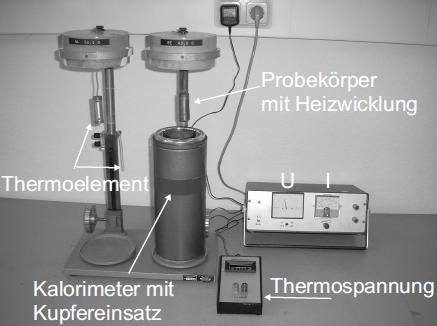
\includegraphics{Aufbau}
	\caption{Aufbau nach \cite[23.4.15, 13 Uhr]{lp25}}
	\label{fig:aufbau}
\end{figure}

In diesem Versuch soll von zwei verschiedenen Körpern der Temperaturverlauf bei der Erwärmung gemessen werden.
Dazu werden zwei Kalorimeter verwendet, welche aus einem Probekörper mit Heizdraht bestehen.
Zuerst werden von den zwei Kalorimetern aus Abb. \ref{fig:aufbau} die Werte der Temperatur bei Raumtemperatur gemessen.
Dies wird je 5 min lang gemacht alle 30 Sekunden.

Anschließend werden die Probekörper mit einem Heizstrom von $0.5\si\volt$ über 15 min erwärmt und dabei ebenfalls alle 30 min die Temperatur aber auch die Spannung, welche benötigt wird um den Strom aufrecht zu erhalten, aufgezeichnet.
Die Spannung muss ständig nachreguliert werden.
Folgend wird über weitere 10 min der Abkühlvorgang protokolliert.

Ist dies beendet, so wird das Isolationsgefäß von dem Tutor mit flüssigem Stickstoff soweit befüllt, dass das Kupfergefäß noch sicher stehen kann.
Die Probekörper werden in die Kupfergefäße gehängt und diese werden so hoch gestellt, dass sie verschlossen werden.
Nun muss solange gewartet werden, bis sich die Temperatur  nicht mehr wesentlich ändert.
Da dies sehr lange dauert, ist zu empfehlen, erst einen Körper zu erheizen und während man diese Messung bei dem Zweiten durchführt schon den ersten herabzukühlen.
Der Probekörper darf jedoch nicht in den Stickstoff gelangen.\newline

Achtung! In diesem Versuch wird mit flüssigem Stickstoff hantiert.
Bei Berührungen mit der Haut kann es zu schweren Verbrennungen kommen.

\section{Auswertung}
\label{sec:auswertung}
\subsection{Temperaturverläufe}
Das Thermoelement gibt eine Spannung in Millivolt zurück.
Diese kann man mit der folgenden Formel und ihrer Fehlerformel in eine Temperatur umrechnen:
\begin{align}
	T[\si{\celsius}]&=0.219+20.456 \cdot U - 0.302\cdot U^2+0.009\cdot U^3 \,, \\
	\sigma_T&=(20.456 - 0.604\cdot U+0.027\cdot U^2)\cdot \sigma_U\,.
\end{align}
Dabei nehmen wir eine Ungenauigkeit von $\sigma_U=0.02\,$mV an.
Diese Temperaturen werden anschließend in Kelvin umgerechnet: $0\si\celsius\corresponds 273.15 \, \si\kelvin$ und $1000\si\celsius\corresponds 373.15 \, \si\kelvin$. 
In Abbildung \ref{fig:Raumtemp} und \ref{fig:Stickstofftemp} ist die Temperatur der beiden Materialien Aluminium und Beryllium gegen die Zeit aufgetragen -- zuerst für Raumtemperatur, dann für Stickstofftemperatur.
Man kann gut erkennen, wann geheizt wurde und wann sich der Körper wieder abkühlt.
Für die Stickstofftemperatur-Messung von Beryllium wurde der Referenzkontakt nicht in Eiswasser getaucht.
Deshalb ist die Referenztemperatur nicht $0\si\celsius$, sondern Raumtemperatur $T(0.88)=18\si\celsius$.
\begin{figure}[!htb]
	\centering
	% GNUPLOT: LaTeX picture with Postscript
\begingroup
  \makeatletter
  \providecommand\color[2][]{%
    \GenericError{(gnuplot) \space\space\space\@spaces}{%
      Package color not loaded in conjunction with
      terminal option `colourtext'%
    }{See the gnuplot documentation for explanation.%
    }{Either use 'blacktext' in gnuplot or load the package
      color.sty in LaTeX.}%
    \renewcommand\color[2][]{}%
  }%
  \providecommand\includegraphics[2][]{%
    \GenericError{(gnuplot) \space\space\space\@spaces}{%
      Package graphicx or graphics not loaded%
    }{See the gnuplot documentation for explanation.%
    }{The gnuplot epslatex terminal needs graphicx.sty or graphics.sty.}%
    \renewcommand\includegraphics[2][]{}%
  }%
  \providecommand\rotatebox[2]{#2}%
  \@ifundefined{ifGPcolor}{%
    \newif\ifGPcolor
    \GPcolortrue
  }{}%
  \@ifundefined{ifGPblacktext}{%
    \newif\ifGPblacktext
    \GPblacktexttrue
  }{}%
  % define a \g@addto@macro without @ in the name:
  \let\gplgaddtomacro\g@addto@macro
  % define empty templates for all commands taking text:
  \gdef\gplbacktext{}%
  \gdef\gplfronttext{}%
  \makeatother
  \ifGPblacktext
    % no textcolor at all
    \def\colorrgb#1{}%
    \def\colorgray#1{}%
  \else
    % gray or color?
    \ifGPcolor
      \def\colorrgb#1{\color[rgb]{#1}}%
      \def\colorgray#1{\color[gray]{#1}}%
      \expandafter\def\csname LTw\endcsname{\color{white}}%
      \expandafter\def\csname LTb\endcsname{\color{black}}%
      \expandafter\def\csname LTa\endcsname{\color{black}}%
      \expandafter\def\csname LT0\endcsname{\color[rgb]{1,0,0}}%
      \expandafter\def\csname LT1\endcsname{\color[rgb]{0,1,0}}%
      \expandafter\def\csname LT2\endcsname{\color[rgb]{0,0,1}}%
      \expandafter\def\csname LT3\endcsname{\color[rgb]{1,0,1}}%
      \expandafter\def\csname LT4\endcsname{\color[rgb]{0,1,1}}%
      \expandafter\def\csname LT5\endcsname{\color[rgb]{1,1,0}}%
      \expandafter\def\csname LT6\endcsname{\color[rgb]{0,0,0}}%
      \expandafter\def\csname LT7\endcsname{\color[rgb]{1,0.3,0}}%
      \expandafter\def\csname LT8\endcsname{\color[rgb]{0.5,0.5,0.5}}%
    \else
      % gray
      \def\colorrgb#1{\color{black}}%
      \def\colorgray#1{\color[gray]{#1}}%
      \expandafter\def\csname LTw\endcsname{\color{white}}%
      \expandafter\def\csname LTb\endcsname{\color{black}}%
      \expandafter\def\csname LTa\endcsname{\color{black}}%
      \expandafter\def\csname LT0\endcsname{\color{black}}%
      \expandafter\def\csname LT1\endcsname{\color{black}}%
      \expandafter\def\csname LT2\endcsname{\color{black}}%
      \expandafter\def\csname LT3\endcsname{\color{black}}%
      \expandafter\def\csname LT4\endcsname{\color{black}}%
      \expandafter\def\csname LT5\endcsname{\color{black}}%
      \expandafter\def\csname LT6\endcsname{\color{black}}%
      \expandafter\def\csname LT7\endcsname{\color{black}}%
      \expandafter\def\csname LT8\endcsname{\color{black}}%
    \fi
  \fi
  \setlength{\unitlength}{0.0500bp}%
  \begin{picture}(7200.00,5040.00)%
    \gplgaddtomacro\gplbacktext{%
      \csname LTb\endcsname%
      \put(946,704){\makebox(0,0)[r]{\strut{} 290}}%
      \put(946,1286){\makebox(0,0)[r]{\strut{} 300}}%
      \put(946,1867){\makebox(0,0)[r]{\strut{} 310}}%
      \put(946,2449){\makebox(0,0)[r]{\strut{} 320}}%
      \put(946,3030){\makebox(0,0)[r]{\strut{} 330}}%
      \put(946,3612){\makebox(0,0)[r]{\strut{} 340}}%
      \put(946,4193){\makebox(0,0)[r]{\strut{} 350}}%
      \put(946,4775){\makebox(0,0)[r]{\strut{} 360}}%
      \put(1078,484){\makebox(0,0){\strut{} 0}}%
      \put(1794,484){\makebox(0,0){\strut{} 2}}%
      \put(2509,484){\makebox(0,0){\strut{} 4}}%
      \put(3225,484){\makebox(0,0){\strut{} 6}}%
      \put(3941,484){\makebox(0,0){\strut{} 8}}%
      \put(4656,484){\makebox(0,0){\strut{} 10}}%
      \put(5372,484){\makebox(0,0){\strut{} 12}}%
      \put(6087,484){\makebox(0,0){\strut{} 14}}%
      \put(6803,484){\makebox(0,0){\strut{} 16}}%
      \put(176,2739){\rotatebox{-270}{\makebox(0,0){\strut{}Temperatur $T$ [$\si\kelvin$]}}}%
      \put(3940,154){\makebox(0,0){\strut{}Zeit $t$ [min]}}%
    }%
    \gplgaddtomacro\gplfronttext{%
      \csname LTb\endcsname%
      \put(5816,4602){\makebox(0,0)[r]{\strut{}Aluminium}}%
      \csname LTb\endcsname%
      \put(5816,4382){\makebox(0,0)[r]{\strut{}Beryllium}}%
    }%
    \gplbacktext
    \put(0,0){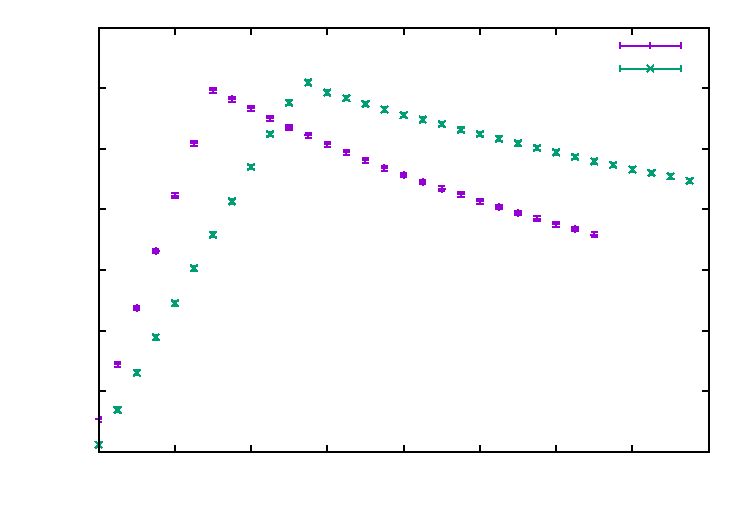
\includegraphics{Raumtemp}}%
    \gplfronttext
  \end{picture}%
\endgroup

	\caption{Raumtemperatur: Erhitzen und Abkühlen von Aluminium und Beryllium}
	\label{fig:Raumtemp}
\end{figure}

\begin{figure}[!htb]
	\centering
	% GNUPLOT: LaTeX picture with Postscript
\begingroup
  \makeatletter
  \providecommand\color[2][]{%
    \GenericError{(gnuplot) \space\space\space\@spaces}{%
      Package color not loaded in conjunction with
      terminal option `colourtext'%
    }{See the gnuplot documentation for explanation.%
    }{Either use 'blacktext' in gnuplot or load the package
      color.sty in LaTeX.}%
    \renewcommand\color[2][]{}%
  }%
  \providecommand\includegraphics[2][]{%
    \GenericError{(gnuplot) \space\space\space\@spaces}{%
      Package graphicx or graphics not loaded%
    }{See the gnuplot documentation for explanation.%
    }{The gnuplot epslatex terminal needs graphicx.sty or graphics.sty.}%
    \renewcommand\includegraphics[2][]{}%
  }%
  \providecommand\rotatebox[2]{#2}%
  \@ifundefined{ifGPcolor}{%
    \newif\ifGPcolor
    \GPcolortrue
  }{}%
  \@ifundefined{ifGPblacktext}{%
    \newif\ifGPblacktext
    \GPblacktexttrue
  }{}%
  % define a \g@addto@macro without @ in the name:
  \let\gplgaddtomacro\g@addto@macro
  % define empty templates for all commands taking text:
  \gdef\gplbacktext{}%
  \gdef\gplfronttext{}%
  \makeatother
  \ifGPblacktext
    % no textcolor at all
    \def\colorrgb#1{}%
    \def\colorgray#1{}%
  \else
    % gray or color?
    \ifGPcolor
      \def\colorrgb#1{\color[rgb]{#1}}%
      \def\colorgray#1{\color[gray]{#1}}%
      \expandafter\def\csname LTw\endcsname{\color{white}}%
      \expandafter\def\csname LTb\endcsname{\color{black}}%
      \expandafter\def\csname LTa\endcsname{\color{black}}%
      \expandafter\def\csname LT0\endcsname{\color[rgb]{1,0,0}}%
      \expandafter\def\csname LT1\endcsname{\color[rgb]{0,1,0}}%
      \expandafter\def\csname LT2\endcsname{\color[rgb]{0,0,1}}%
      \expandafter\def\csname LT3\endcsname{\color[rgb]{1,0,1}}%
      \expandafter\def\csname LT4\endcsname{\color[rgb]{0,1,1}}%
      \expandafter\def\csname LT5\endcsname{\color[rgb]{1,1,0}}%
      \expandafter\def\csname LT6\endcsname{\color[rgb]{0,0,0}}%
      \expandafter\def\csname LT7\endcsname{\color[rgb]{1,0.3,0}}%
      \expandafter\def\csname LT8\endcsname{\color[rgb]{0.5,0.5,0.5}}%
    \else
      % gray
      \def\colorrgb#1{\color{black}}%
      \def\colorgray#1{\color[gray]{#1}}%
      \expandafter\def\csname LTw\endcsname{\color{white}}%
      \expandafter\def\csname LTb\endcsname{\color{black}}%
      \expandafter\def\csname LTa\endcsname{\color{black}}%
      \expandafter\def\csname LT0\endcsname{\color{black}}%
      \expandafter\def\csname LT1\endcsname{\color{black}}%
      \expandafter\def\csname LT2\endcsname{\color{black}}%
      \expandafter\def\csname LT3\endcsname{\color{black}}%
      \expandafter\def\csname LT4\endcsname{\color{black}}%
      \expandafter\def\csname LT5\endcsname{\color{black}}%
      \expandafter\def\csname LT6\endcsname{\color{black}}%
      \expandafter\def\csname LT7\endcsname{\color{black}}%
      \expandafter\def\csname LT8\endcsname{\color{black}}%
    \fi
  \fi
    \setlength{\unitlength}{0.0500bp}%
    \ifx\gptboxheight\undefined%
      \newlength{\gptboxheight}%
      \newlength{\gptboxwidth}%
      \newsavebox{\gptboxtext}%
    \fi%
    \setlength{\fboxrule}{0.5pt}%
    \setlength{\fboxsep}{1pt}%
\begin{picture}(7200.00,5040.00)%
    \gplgaddtomacro\gplbacktext{%
      \csname LTb\endcsname%
      \put(946,704){\makebox(0,0)[r]{\strut{}$-180$}}%
      \put(946,1382){\makebox(0,0)[r]{\strut{}$-160$}}%
      \put(946,2061){\makebox(0,0)[r]{\strut{}$-140$}}%
      \put(946,2739){\makebox(0,0)[r]{\strut{}$-120$}}%
      \put(946,3418){\makebox(0,0)[r]{\strut{}$-100$}}%
      \put(946,4096){\makebox(0,0)[r]{\strut{}$-80$}}%
      \put(946,4775){\makebox(0,0)[r]{\strut{}$-60$}}%
      \put(1078,484){\makebox(0,0){\strut{}$0$}}%
      \put(2223,484){\makebox(0,0){\strut{}$5$}}%
      \put(3368,484){\makebox(0,0){\strut{}$10$}}%
      \put(4513,484){\makebox(0,0){\strut{}$15$}}%
      \put(5658,484){\makebox(0,0){\strut{}$20$}}%
      \put(6803,484){\makebox(0,0){\strut{}$25$}}%
    }%
    \gplgaddtomacro\gplfronttext{%
      \csname LTb\endcsname%
      \put(176,2739){\rotatebox{-270}{\makebox(0,0){\strut{}Temperatur $T$ [$^\circ C$]}}}%
      \put(3940,154){\makebox(0,0){\strut{}Zeit $t$ [min]}}%
      \csname LTb\endcsname%
      \put(5816,4602){\makebox(0,0)[r]{\strut{}Aluminium}}%
      \csname LTb\endcsname%
      \put(5816,4382){\makebox(0,0)[r]{\strut{}Beryllium}}%
    }%
    \gplbacktext
    \put(0,0){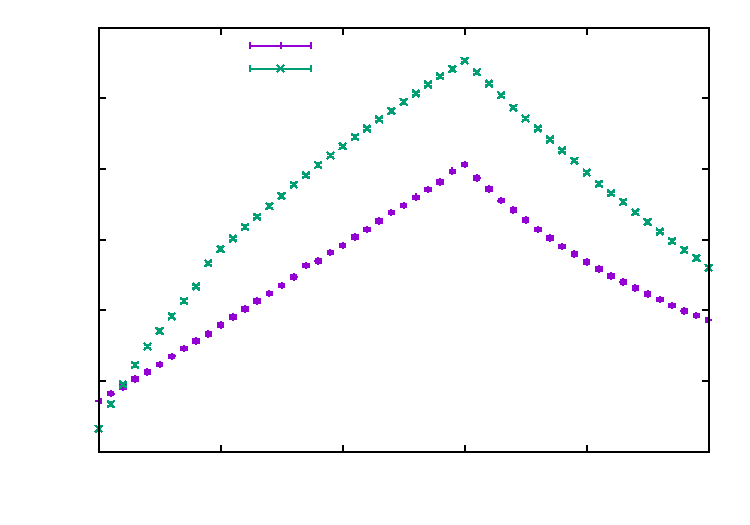
\includegraphics{Stickstofftemp}}%
    \gplfronttext
  \end{picture}%
\endgroup

	\caption{Stickstofftemperatur: Erhitzen und Abkühlen von Aluminium und Beryllium}
	\label{fig:Stickstofftemp}
\end{figure}

\subsection{Widerstand}
Den Widerstand des Kupferdrahtes kann man leicht berechnen, indem man die Heizspannung $U$ durch die Stromstärke $I$, die konstant bei$0.5\,$A liegt, teilt:
\begin{align}
	R&=\frac{U}{I}\,,\\
	\sigma_R&=\frac{\sigma_U}{I}\,.
\end{align}
Wir nehmen einen Fehler der Heizspannung von $\sigma_U=0.4\,$V an, da sich die Spannung während 30 Sekunden stark ändern konnte.
Wenn die Spannung mit dem Schalter verdreifacht wurde, verdreifacht sich der Fehler auch auf $\sigma_U=1.2\,$V.
In Abb.\ref{fig:Widerstand} ist der Widerstand des Drahtes während der vier Heizvorgänge gegen die Temperatur aufgetragen.
\begin{figure}[!htb]
	\centering
	% GNUPLOT: LaTeX picture with Postscript
\begingroup
  \makeatletter
  \providecommand\color[2][]{%
    \GenericError{(gnuplot) \space\space\space\@spaces}{%
      Package color not loaded in conjunction with
      terminal option `colourtext'%
    }{See the gnuplot documentation for explanation.%
    }{Either use 'blacktext' in gnuplot or load the package
      color.sty in LaTeX.}%
    \renewcommand\color[2][]{}%
  }%
  \providecommand\includegraphics[2][]{%
    \GenericError{(gnuplot) \space\space\space\@spaces}{%
      Package graphicx or graphics not loaded%
    }{See the gnuplot documentation for explanation.%
    }{The gnuplot epslatex terminal needs graphicx.sty or graphics.sty.}%
    \renewcommand\includegraphics[2][]{}%
  }%
  \providecommand\rotatebox[2]{#2}%
  \@ifundefined{ifGPcolor}{%
    \newif\ifGPcolor
    \GPcolortrue
  }{}%
  \@ifundefined{ifGPblacktext}{%
    \newif\ifGPblacktext
    \GPblacktexttrue
  }{}%
  % define a \g@addto@macro without @ in the name:
  \let\gplgaddtomacro\g@addto@macro
  % define empty templates for all commands taking text:
  \gdef\gplbacktext{}%
  \gdef\gplfronttext{}%
  \makeatother
  \ifGPblacktext
    % no textcolor at all
    \def\colorrgb#1{}%
    \def\colorgray#1{}%
  \else
    % gray or color?
    \ifGPcolor
      \def\colorrgb#1{\color[rgb]{#1}}%
      \def\colorgray#1{\color[gray]{#1}}%
      \expandafter\def\csname LTw\endcsname{\color{white}}%
      \expandafter\def\csname LTb\endcsname{\color{black}}%
      \expandafter\def\csname LTa\endcsname{\color{black}}%
      \expandafter\def\csname LT0\endcsname{\color[rgb]{1,0,0}}%
      \expandafter\def\csname LT1\endcsname{\color[rgb]{0,1,0}}%
      \expandafter\def\csname LT2\endcsname{\color[rgb]{0,0,1}}%
      \expandafter\def\csname LT3\endcsname{\color[rgb]{1,0,1}}%
      \expandafter\def\csname LT4\endcsname{\color[rgb]{0,1,1}}%
      \expandafter\def\csname LT5\endcsname{\color[rgb]{1,1,0}}%
      \expandafter\def\csname LT6\endcsname{\color[rgb]{0,0,0}}%
      \expandafter\def\csname LT7\endcsname{\color[rgb]{1,0.3,0}}%
      \expandafter\def\csname LT8\endcsname{\color[rgb]{0.5,0.5,0.5}}%
    \else
      % gray
      \def\colorrgb#1{\color{black}}%
      \def\colorgray#1{\color[gray]{#1}}%
      \expandafter\def\csname LTw\endcsname{\color{white}}%
      \expandafter\def\csname LTb\endcsname{\color{black}}%
      \expandafter\def\csname LTa\endcsname{\color{black}}%
      \expandafter\def\csname LT0\endcsname{\color{black}}%
      \expandafter\def\csname LT1\endcsname{\color{black}}%
      \expandafter\def\csname LT2\endcsname{\color{black}}%
      \expandafter\def\csname LT3\endcsname{\color{black}}%
      \expandafter\def\csname LT4\endcsname{\color{black}}%
      \expandafter\def\csname LT5\endcsname{\color{black}}%
      \expandafter\def\csname LT6\endcsname{\color{black}}%
      \expandafter\def\csname LT7\endcsname{\color{black}}%
      \expandafter\def\csname LT8\endcsname{\color{black}}%
    \fi
  \fi
  \setlength{\unitlength}{0.0500bp}%
  \begin{picture}(7200.00,5040.00)%
    \gplgaddtomacro\gplbacktext{%
      \csname LTb\endcsname%
      \put(814,704){\makebox(0,0)[r]{\strut{} 10}}%
      \put(814,1213){\makebox(0,0)[r]{\strut{} 20}}%
      \put(814,1722){\makebox(0,0)[r]{\strut{} 30}}%
      \put(814,2231){\makebox(0,0)[r]{\strut{} 40}}%
      \put(814,2740){\makebox(0,0)[r]{\strut{} 50}}%
      \put(814,3248){\makebox(0,0)[r]{\strut{} 60}}%
      \put(814,3757){\makebox(0,0)[r]{\strut{} 70}}%
      \put(814,4266){\makebox(0,0)[r]{\strut{} 80}}%
      \put(814,4775){\makebox(0,0)[r]{\strut{} 90}}%
      \put(946,484){\makebox(0,0){\strut{} 100}}%
      \put(2117,484){\makebox(0,0){\strut{} 150}}%
      \put(3289,484){\makebox(0,0){\strut{} 200}}%
      \put(4460,484){\makebox(0,0){\strut{} 250}}%
      \put(5632,484){\makebox(0,0){\strut{} 300}}%
      \put(6803,484){\makebox(0,0){\strut{} 350}}%
      \put(176,2739){\rotatebox{-270}{\makebox(0,0){\strut{}Widerstand $R$  [$\Omega$]}}}%
      \put(3874,154){\makebox(0,0){\strut{}Temperatur $T$ [$\si\kelvin$]}}%
    }%
    \gplgaddtomacro\gplfronttext{%
      \csname LTb\endcsname%
      \put(2266,4602){\makebox(0,0)[r]{\strut{}Aluminium}}%
      \csname LTb\endcsname%
      \put(2266,4382){\makebox(0,0)[r]{\strut{}Beryllium}}%
    }%
    \gplbacktext
    \put(0,0){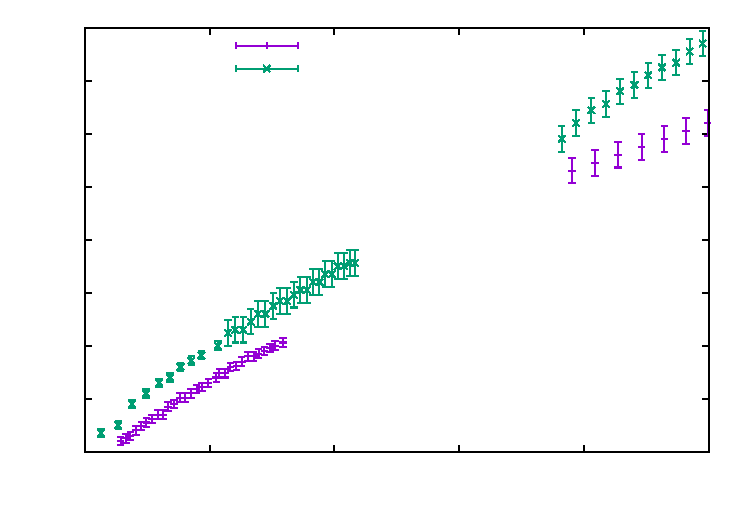
\includegraphics{Widerstand}}%
    \gplfronttext
  \end{picture}%
\endgroup

	\caption{Widerstand des Cu-Drahtes}
	\label{fig:Widerstand}
\end{figure}

\subsection{Leistung}
Die Heizleistung kann man mit der Folgenden Formel und ihrer Fehlerformel berechnet werden:
\begin{align}
	P&=UI\,,\\
	\sigma_P&=I\cdot\sigma_U\,.
\end{align}
Es wird der gleiche Fehler $\sigma_U$ wie zuvor auch verwendet.
Nun kann die elektrische Leistung während des Heizvorgangs gegen die Temperatur aufgetragen werden (vgl. Abb.\ref{fig:Leistung}).
\begin{figure}[!htb]
	\centering
	% GNUPLOT: LaTeX picture with Postscript
\begingroup
  \makeatletter
  \providecommand\color[2][]{%
    \GenericError{(gnuplot) \space\space\space\@spaces}{%
      Package color not loaded in conjunction with
      terminal option `colourtext'%
    }{See the gnuplot documentation for explanation.%
    }{Either use 'blacktext' in gnuplot or load the package
      color.sty in LaTeX.}%
    \renewcommand\color[2][]{}%
  }%
  \providecommand\includegraphics[2][]{%
    \GenericError{(gnuplot) \space\space\space\@spaces}{%
      Package graphicx or graphics not loaded%
    }{See the gnuplot documentation for explanation.%
    }{The gnuplot epslatex terminal needs graphicx.sty or graphics.sty.}%
    \renewcommand\includegraphics[2][]{}%
  }%
  \providecommand\rotatebox[2]{#2}%
  \@ifundefined{ifGPcolor}{%
    \newif\ifGPcolor
    \GPcolortrue
  }{}%
  \@ifundefined{ifGPblacktext}{%
    \newif\ifGPblacktext
    \GPblacktexttrue
  }{}%
  % define a \g@addto@macro without @ in the name:
  \let\gplgaddtomacro\g@addto@macro
  % define empty templates for all commands taking text:
  \gdef\gplbacktext{}%
  \gdef\gplfronttext{}%
  \makeatother
  \ifGPblacktext
    % no textcolor at all
    \def\colorrgb#1{}%
    \def\colorgray#1{}%
  \else
    % gray or color?
    \ifGPcolor
      \def\colorrgb#1{\color[rgb]{#1}}%
      \def\colorgray#1{\color[gray]{#1}}%
      \expandafter\def\csname LTw\endcsname{\color{white}}%
      \expandafter\def\csname LTb\endcsname{\color{black}}%
      \expandafter\def\csname LTa\endcsname{\color{black}}%
      \expandafter\def\csname LT0\endcsname{\color[rgb]{1,0,0}}%
      \expandafter\def\csname LT1\endcsname{\color[rgb]{0,1,0}}%
      \expandafter\def\csname LT2\endcsname{\color[rgb]{0,0,1}}%
      \expandafter\def\csname LT3\endcsname{\color[rgb]{1,0,1}}%
      \expandafter\def\csname LT4\endcsname{\color[rgb]{0,1,1}}%
      \expandafter\def\csname LT5\endcsname{\color[rgb]{1,1,0}}%
      \expandafter\def\csname LT6\endcsname{\color[rgb]{0,0,0}}%
      \expandafter\def\csname LT7\endcsname{\color[rgb]{1,0.3,0}}%
      \expandafter\def\csname LT8\endcsname{\color[rgb]{0.5,0.5,0.5}}%
    \else
      % gray
      \def\colorrgb#1{\color{black}}%
      \def\colorgray#1{\color[gray]{#1}}%
      \expandafter\def\csname LTw\endcsname{\color{white}}%
      \expandafter\def\csname LTb\endcsname{\color{black}}%
      \expandafter\def\csname LTa\endcsname{\color{black}}%
      \expandafter\def\csname LT0\endcsname{\color{black}}%
      \expandafter\def\csname LT1\endcsname{\color{black}}%
      \expandafter\def\csname LT2\endcsname{\color{black}}%
      \expandafter\def\csname LT3\endcsname{\color{black}}%
      \expandafter\def\csname LT4\endcsname{\color{black}}%
      \expandafter\def\csname LT5\endcsname{\color{black}}%
      \expandafter\def\csname LT6\endcsname{\color{black}}%
      \expandafter\def\csname LT7\endcsname{\color{black}}%
      \expandafter\def\csname LT8\endcsname{\color{black}}%
    \fi
  \fi
  \setlength{\unitlength}{0.0500bp}%
  \begin{picture}(7200.00,5040.00)%
    \gplgaddtomacro\gplbacktext{%
      \csname LTb\endcsname%
      \put(814,704){\makebox(0,0)[r]{\strut{} 2}}%
      \put(814,1074){\makebox(0,0)[r]{\strut{} 4}}%
      \put(814,1444){\makebox(0,0)[r]{\strut{} 6}}%
      \put(814,1814){\makebox(0,0)[r]{\strut{} 8}}%
      \put(814,2184){\makebox(0,0)[r]{\strut{} 10}}%
      \put(814,2554){\makebox(0,0)[r]{\strut{} 12}}%
      \put(814,2925){\makebox(0,0)[r]{\strut{} 14}}%
      \put(814,3295){\makebox(0,0)[r]{\strut{} 16}}%
      \put(814,3665){\makebox(0,0)[r]{\strut{} 18}}%
      \put(814,4035){\makebox(0,0)[r]{\strut{} 20}}%
      \put(814,4405){\makebox(0,0)[r]{\strut{} 22}}%
      \put(814,4775){\makebox(0,0)[r]{\strut{} 24}}%
      \put(946,484){\makebox(0,0){\strut{} 100}}%
      \put(2117,484){\makebox(0,0){\strut{} 150}}%
      \put(3289,484){\makebox(0,0){\strut{} 200}}%
      \put(4460,484){\makebox(0,0){\strut{} 250}}%
      \put(5632,484){\makebox(0,0){\strut{} 300}}%
      \put(6803,484){\makebox(0,0){\strut{} 350}}%
      \put(176,2739){\rotatebox{-270}{\makebox(0,0){\strut{}Leistung $P$  [W]}}}%
      \put(3874,154){\makebox(0,0){\strut{}Temperatur $T$ [$\si\kelvin$]}}%
    }%
    \gplgaddtomacro\gplfronttext{%
      \csname LTb\endcsname%
      \put(2266,4602){\makebox(0,0)[r]{\strut{}Aluminium}}%
      \csname LTb\endcsname%
      \put(2266,4382){\makebox(0,0)[r]{\strut{}Beryllium}}%
    }%
    \gplbacktext
    \put(0,0){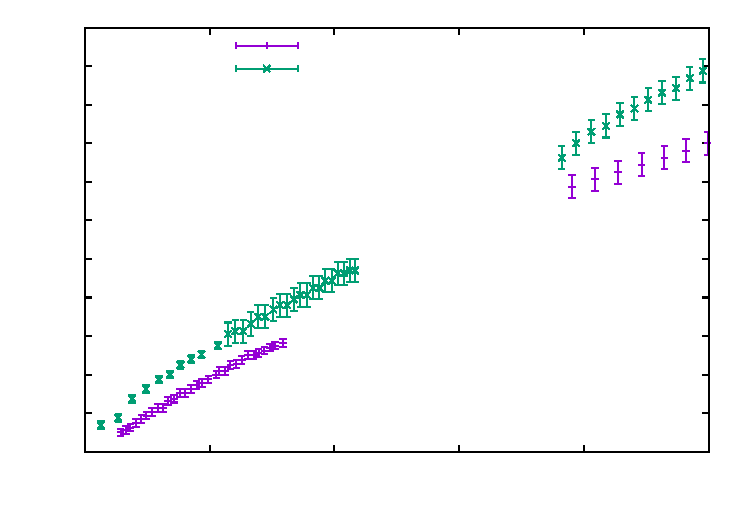
\includegraphics{Leistung}}%
    \gplfronttext
  \end{picture}%
\endgroup

	\caption{Beim Heizen hineingesteckte Leistung}
	\label{fig:Leistung}
\end{figure}

\subsection{molare Wärmekapazität}
Für das Erwärmen wird ein linearer Zusammenhang zwischen Temperatur und Zeit erwartet: $T(t)=a\cdot t +b$.
Dann ist $\frac{\dif T}{\dif t}|_\text{erw}=a$.
Für das Abkühlen kann man einen exponentiellen Abfall der Temperatur mit der Zeit annehmen.
Zudem wird sich die Temperatur dem thermischen Gleichgewicht angleichen: $T(t)=T_0+(T_1-T_0)\cdot e^{-\lambda t}$.
Somit ist $\frac{\dif T}{\dif t}|_\text{abk}=-\lambda\cdot (T-T_0)$.
Dabei ist $T_0$ die Temperatur des thermischen Gleichgewichtes.
Setzt man dies für die molare Wärmekapazität nach \eqref{eq:molWaerme} ein, ergibt sich
\begin{align}
	c_m&=\frac{M}{m}\frac{P}{a+\lambda (T-T_0)}
	\label{eq:c_m}\\
	\sigma{c_m}&=\frac{M}{m}\sqrt{\frac{\sigma_P^2}{(a+\lambda (T-T_0))^2}+\frac{P^2}{(a+\lambda (T-T_0))^4}\cdot (\sigma_a^2+(T-T_0)^2 \sigma_\lambda^2+\lambda^2\sigma_T^2)}\,.
	\label{eq:sigma_c_m}
\end{align}
Die molare Masse von Aluminium beträgt $M=26.982\,\si{\gram\per\mol}$, von Beryllium $M=9.012\,\si{\gram\per\mol}$.
Die Masse des Aluminium-Körpers ist $m=52.5\,\si\gram$, die des Beryllium-Körpers ist $m=43.0\,\si\gram$.\\
Um die Temperatur $T_0$ zu ermitteln, werden die Werte vor dem Erhitzen verwendet.
Diese waren bei Zimmertemperatur erwartungsgemäß konstant.
Somit liegt die Zimmertemperatur bei $T_0(0.88\,\text{mV})=18\si{\celsius}$.
Bei dem zweiten Versuchsteil wurde vor dem Erhitzen noch nicht das thermische Gleichgewicht erreicht.
Man nimmt wieder an, dass sich die Temperatur exponentiell abfallend an die Gleichgewichtstemperatur nähert.
Mit einem $\chi^2$-Fit ergibt sich für die Versuchsreihe mit Aluminium $T_0=110\si\celsius$, für die mit Beryllium $T_0=106\si\celsius$.
So kann man jetzt $\lambda$ bestimmen, indem man die Temperaturdifferenz zu $T_0$ während des Abkühlvorgangs logarithmisch gegen die Zeit aufträgt.
Es ergibt sich eine Gerade, deren Steigung mit einer linearen Regression bestimmt werden kann.
Die Werte für $a$ und $\lambda$ der 4 Versuchsreihen befinden sich in Tabelle \ref{tab:fitwerte}.
\begin{table}[!htb]
	\centering
	\begin{tabular}{|c|c|c|}
		\hline
		& $a~[10^{-3} \cdot \si{\kelvin\per\second}]$ & $\lambda~[10^{-5} \cdot \si{\per\second}]$\\
		\hline
		Al RT	& $	303	\pm	2	$ & $	87.8	\pm	0.6	$ \\
		Be RT	& $	188.5	\pm	1.2	$ & $	51.4	\pm	0.6	$ \\
		Al Stickstoff	& $	74.85	\pm	0.23	$ & $	158.8 \pm 0.4	$ \\
		Be Stickstoff	& $	109	\pm	4	$ & $	171 \pm 5$ \\
		\hline
	\end{tabular}
	\caption{Temperaturverläufe: gefittete Parameter}
	\label{tab:fitwerte}
\end{table}
Mit diesen und Formel \eqref{eq:c_m} sowie \eqref{eq:sigma_c_m} kann man nun die molare Wärme berechnen und gegen die Temperatur auftragen (vgl. Abb.\ref{fig:molWaerme}).
Nach Dulong-Petit sollte sich der konstante Wert $3R$ ergeben, nach dem Debye-Modell erwartet man einen Verlauf nach \eqref{eq:debye}.
Dabei liegt die Debye-Temperatur nach \cite[S.226]{prakti} für Aluminium bei $\theta_D=428\,\si\kelvin$, für Beryllium bei $\theta_D=1440\,\si\kelvin$.

\begin{figure}[!htb]
	\centering
	% GNUPLOT: LaTeX picture with Postscript
\begingroup
  \makeatletter
  \providecommand\color[2][]{%
    \GenericError{(gnuplot) \space\space\space\@spaces}{%
      Package color not loaded in conjunction with
      terminal option `colourtext'%
    }{See the gnuplot documentation for explanation.%
    }{Either use 'blacktext' in gnuplot or load the package
      color.sty in LaTeX.}%
    \renewcommand\color[2][]{}%
  }%
  \providecommand\includegraphics[2][]{%
    \GenericError{(gnuplot) \space\space\space\@spaces}{%
      Package graphicx or graphics not loaded%
    }{See the gnuplot documentation for explanation.%
    }{The gnuplot epslatex terminal needs graphicx.sty or graphics.sty.}%
    \renewcommand\includegraphics[2][]{}%
  }%
  \providecommand\rotatebox[2]{#2}%
  \@ifundefined{ifGPcolor}{%
    \newif\ifGPcolor
    \GPcolortrue
  }{}%
  \@ifundefined{ifGPblacktext}{%
    \newif\ifGPblacktext
    \GPblacktexttrue
  }{}%
  % define a \g@addto@macro without @ in the name:
  \let\gplgaddtomacro\g@addto@macro
  % define empty templates for all commands taking text:
  \gdef\gplbacktext{}%
  \gdef\gplfronttext{}%
  \makeatother
  \ifGPblacktext
    % no textcolor at all
    \def\colorrgb#1{}%
    \def\colorgray#1{}%
  \else
    % gray or color?
    \ifGPcolor
      \def\colorrgb#1{\color[rgb]{#1}}%
      \def\colorgray#1{\color[gray]{#1}}%
      \expandafter\def\csname LTw\endcsname{\color{white}}%
      \expandafter\def\csname LTb\endcsname{\color{black}}%
      \expandafter\def\csname LTa\endcsname{\color{black}}%
      \expandafter\def\csname LT0\endcsname{\color[rgb]{1,0,0}}%
      \expandafter\def\csname LT1\endcsname{\color[rgb]{0,1,0}}%
      \expandafter\def\csname LT2\endcsname{\color[rgb]{0,0,1}}%
      \expandafter\def\csname LT3\endcsname{\color[rgb]{1,0,1}}%
      \expandafter\def\csname LT4\endcsname{\color[rgb]{0,1,1}}%
      \expandafter\def\csname LT5\endcsname{\color[rgb]{1,1,0}}%
      \expandafter\def\csname LT6\endcsname{\color[rgb]{0,0,0}}%
      \expandafter\def\csname LT7\endcsname{\color[rgb]{1,0.3,0}}%
      \expandafter\def\csname LT8\endcsname{\color[rgb]{0.5,0.5,0.5}}%
    \else
      % gray
      \def\colorrgb#1{\color{black}}%
      \def\colorgray#1{\color[gray]{#1}}%
      \expandafter\def\csname LTw\endcsname{\color{white}}%
      \expandafter\def\csname LTb\endcsname{\color{black}}%
      \expandafter\def\csname LTa\endcsname{\color{black}}%
      \expandafter\def\csname LT0\endcsname{\color{black}}%
      \expandafter\def\csname LT1\endcsname{\color{black}}%
      \expandafter\def\csname LT2\endcsname{\color{black}}%
      \expandafter\def\csname LT3\endcsname{\color{black}}%
      \expandafter\def\csname LT4\endcsname{\color{black}}%
      \expandafter\def\csname LT5\endcsname{\color{black}}%
      \expandafter\def\csname LT6\endcsname{\color{black}}%
      \expandafter\def\csname LT7\endcsname{\color{black}}%
      \expandafter\def\csname LT8\endcsname{\color{black}}%
    \fi
  \fi
  \setlength{\unitlength}{0.0500bp}%
  \begin{picture}(7200.00,5040.00)%
    \gplgaddtomacro\gplbacktext{%
      \csname LTb\endcsname%
      \put(814,704){\makebox(0,0)[r]{\strut{} 0}}%
      \put(814,1383){\makebox(0,0)[r]{\strut{} 5}}%
      \put(814,2061){\makebox(0,0)[r]{\strut{} 10}}%
      \put(814,2740){\makebox(0,0)[r]{\strut{} 15}}%
      \put(814,3418){\makebox(0,0)[r]{\strut{} 20}}%
      \put(814,4097){\makebox(0,0)[r]{\strut{} 25}}%
      \put(814,4775){\makebox(0,0)[r]{\strut{} 30}}%
      \put(946,484){\makebox(0,0){\strut{} 100}}%
      \put(2117,484){\makebox(0,0){\strut{} 150}}%
      \put(3289,484){\makebox(0,0){\strut{} 200}}%
      \put(4460,484){\makebox(0,0){\strut{} 250}}%
      \put(5632,484){\makebox(0,0){\strut{} 300}}%
      \put(6803,484){\makebox(0,0){\strut{} 350}}%
      \put(176,2739){\rotatebox{-270}{\makebox(0,0){\strut{}molare Wärmekapatität $c_m$  [$\si[per-mode=fraction]{\joule\per\kelvin\per\mol}$]}}}%
      \put(3874,154){\makebox(0,0){\strut{}Temperatur $T$ [K]}}%
    }%
    \gplgaddtomacro\gplfronttext{%
      \csname LTb\endcsname%
      \put(5816,1537){\makebox(0,0)[r]{\strut{}Aluminium}}%
      \csname LTb\endcsname%
      \put(5816,1317){\makebox(0,0)[r]{\strut{}Beryllium}}%
      \csname LTb\endcsname%
      \put(5816,1097){\makebox(0,0)[r]{\strut{}Dulong-Petit-Wert}}%
      \csname LTb\endcsname%
      \put(5816,877){\makebox(0,0)[r]{\strut{}Be: Wert nach Debye}}%
    }%
    \gplbacktext
    \put(0,0){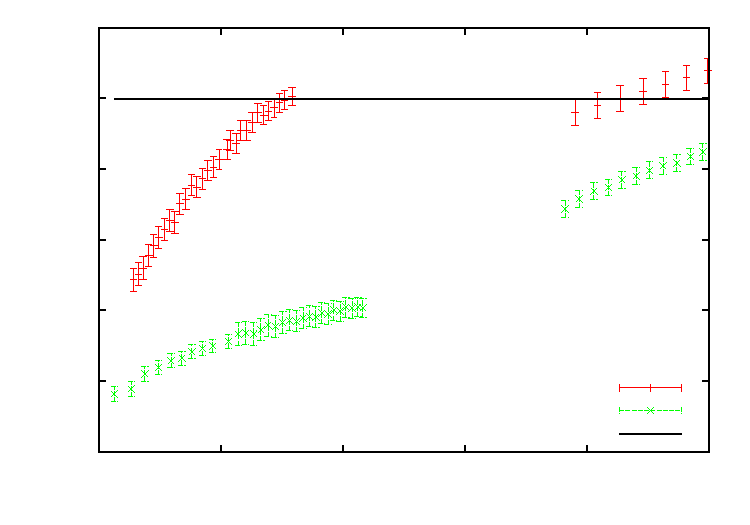
\includegraphics{waerme}}%
    \gplfronttext
  \end{picture}%
\endgroup

	\caption{molare Wärmekapazität bei verschiedenen Temperaturen für Aluminium und Beryllium sowie Vergleich mit dem Dulong-Petit-Wert und den Verläufen nach Debye}
	\label{fig:molWaerme}
\end{figure}

\section{Diskussion}
\label{sec:diskussion}
\subsection{Temperaturverläufe}
Beim Heizen bei Zimmertemperatur (Abb.\ref{fig:Raumtemp})fällt auf, dass die beiden Körper relativ schnell die Maximaltemperatur von $80\si\celsius$ erreichen.
Damit man mehr Messwerte erhält, hätte man in kleineren Zeitintervallen messen müssen oder bei einer kleineren Stromstärke heizen sollen.
Die wenigen Messwerte beeinflussen die Bestimmung der molaren Wärmekapazität eventuell negativ.

An den Temperaturverläufen, die bei Stickstoffkühlung aufgenommen wurden, also Abb.\ref{fig:Stickstofftemp}, kann man erkennen, dass vor Anfang der Messung noch nicht die Siedetemperatur von Stickstoff $-196\si\celsius\corresponds 77.15\,\si\kelvin$ erreicht wurde.
Das thermische Gleichgewicht ist auch nicht erreicht worden.
Um bessere Messwerte zu erhalten, hätte man also noch länger warten müssen oder mehr Stickstoff verwenden müssen.
Der Knick während des Erwärmens von Beryllium in Abb.\ref{fig:Stickstofftemp} lässt sich damit erklären, dass die Heizspannung danach mit dem Schalter verdreifacht wurde und so erstmal kleiner gedreht werden musste.

Bei Beryllium hätte man länger den Abkühlvorgang beobachten müssen, um den erwarteten exponentiellen Abfall an die Gleichgewichtstemperatur zu beobachten.
Die Messwerte sehen nämlich ziemlich linear aus.

\subsection{Widerstand und Leistung}
Bei den Widerstandswerten aus Abb.\ref{fig:Widerstand} erkennt man, dass sie bei dem Aufbau für Aluminium stets geringer sind als bei dem für Beryllium.
Dies lässt sich damit erklären, dass der verwendete Kupferdraht bei Beryllium länger oder dünner ist.
Dies erhöht den Widerstand.
Außerdem ist der Widerstand stark temperaturabhängig.
Interpoliert man den Widerstand bei noch niedrigeren Temperaturen, müsste man einen Punkt erreichen, an dem der Draht keinen Widerstand hat.
Dies zu untersuchen wäre auch interessant gewesen, man hätte dazu aber nicht mehr Stickstoff als Kühlung nehmen können.
Eigentlich sollte der Widerstand erst am absoluten Nullpunkt $0\,$K verschwinden.
Nach den Daten aus Abb.\ref{fig:Widerstand} sieht es aber so aus, als würde er bei drei von vier Messreihen schon bei einer höheren Temperatur verschwinden.
Dies ist ein Hinweis auf einen systematischen Fehler.\\
Ähnliches gilt auch für die Leistung in Abb.\ref{fig:Leistung}.
In der Auswertung wird angenommen, dass die gesamte elektrische Leistung an den Probekörper abgegeben wird.
Sie könnte aber auch an die Umgebung abgegeben werden.
So sollte die tatsächliche Leistung geringer sein. 

\subsection{molare Wärmekapazität}
In Abb.\ref{fig:molWaerme} sind sowohl die Theoriekurven als auch unsere Messwerte für die molare Wärme beider Elemente eingezeichnet.
Bei Zimmertemperatur passen die Werte gut zum Wert nach Dulong-Petit.
Man sieht deutlich, dass die Messwerte immer größer sind, als das Debye-Modell vorhersagt.
Bei den beiden Messreihen von Aluminium sieht es nach einem konstanten Offset aus.
Dieser könnte zum Beispiel durch eine konstant höhere Stromstärke erklärt werden.
Bei der zweiten Messreihe von Beryllium, also gekühlt, wurde der Referenzkontakt nicht in Eiswasser getaucht.
Man kann die Temperatur aber nicht ganz so einfach wie in der Auswertung umrechnen.
Außerdem ist die Raumtemperatur aufgrund des Versuchs nicht konstant.
Sie ist vermutlich gesunken.
Dies konnte aber nicht berücksichtigt werden.
Wegen diesen Messungenauigkeiten ist es auch nicht verwunderlich, dass die Werte nicht ganz zur Theorie passen.\\
Die für tiefe Temperaturen aus dem Debye-Modell abgeleitete Abhängigkeit $c_m\sim \frac{T}{\theta_D}$ kann man erst bei viel tieferen Temperaturen verifizieren, da bei unserer Messung $T \ll \theta_D$ in beiden Fällen nicht galt.
Trotzdem erkennt man, dass die Dulong-Petitsche Regel für den zweiten vermessenen Temperaturbereich nicht gilt.

\bibliography{literatur}
\bibliographystyle{babalpha}

\end{document}
